\documentclass[14pt, a4paper]{extreport}
\usepackage{extsizes}
\usepackage[a4paper, left=30mm, right=15mm, top=20mm, bottom=20mm]{geometry}
\usepackage[english, russian]{babel}
\usepackage{fontspec}
\defaultfontfeatures{Ligatures={TeX},Renderer=Basic}
\setmainfont[Ligatures={TeX,Historic}]{Times New Roman}
\usepackage{amsmath,amssymb}
\usepackage{listings}
\usepackage{graphicx}
\usepackage{setspace}
\graphicspath{{images/}}
\usepackage[hidelinks]{hyperref}
\usepackage{indentfirst}
\setlength{\parindent}{1.25cm}
\usepackage[explicit,compact]{titlesec}
\usepackage{titletoc}
\newcommand{\doublerule}[1][.4pt]{%
	\noindent
	\makebox[0pt][l]{\rule[.6ex]{\linewidth}{#1}}%
	\rule[.3ex]{\linewidth}{#1}
}

\addto\captionsrussian{%
	\renewcommand{\contentsname}%
	{\centering{СОДЕРЖАНИЕ}}%
}

\usepackage{caption}
\DeclareCaptionLabelSeparator{dash}{ -- }
\DeclareCaptionLabelFormat{figure}{Рисунок #2}
\DeclareCaptionFormat{listing}{\hspace*{1.25cm}#1#2#3}
\captionsetup[table]{
	labelsep=dash,
	singlelinecheck=false,
}
\captionsetup[figure]{
	labelsep=dash,
	labelformat=figure,
}
\captionsetup[lstlisting]{
	format=listing,
	labelsep=dash,
	justification=raggedright,
	singlelinecheck=false,
}

\usepackage{floatrow}
\floatsetup[table]{style=plaintop}
\floatsetup[equation]{style=plain}

\usepackage{chngcntr}
\counterwithout{figure}{chapter}
\counterwithout{equation}{chapter}
\counterwithout{table}{chapter}

\usepackage{cleveref}
\crefformat{table}{смотри табл.#2#1#3}
\Crefformat{table}{Смотри табл.#2#1#3}

\crefformat{figure}{рис.~#2#1#3}
\Crefformat{figure}{Рис.~#2#1#3}
\crefmultiformat{figure}{рис.~#2#1#3}{,~#2#1#3}{,~#2#1#3}{,~#2#1#3}
\crefrangeformat{figure}{рис.~#3#1#4--#5#2#6}

\crefformat{equation}{#1}
\crefmultiformat{equation}{~#2#1#3}{,~#2#1#3}{,~#2#1#3}{,~#2#1#3}
\crefrangeformat{equation}{~#3#1#4--#5#2#6}

\crefname{listing}{листингом}{листингами}
\Crefname{listing}{Листингом}{Листингами}
\crefrangeformat{listing}{листингами~#3#1#4--#5#2#6}

\setmonofont{Courier New}[Scale=0.857]
\lstset{basicstyle=\small\ttfamily}

\begin{document}
\counterwithout{lstlisting}{chapter}

\begin{titlepage}
	\begin{center}
		\vspace*{0.5mm}
		\setstretch{1.1}

		
\includegraphics[width=0.18\textwidth]{logo}\\
		\footnotesize
		МИНИСТЕРСТВО НАУКИ И ВЫСШЕГО ОБРАЗОВАНИЯ РОССИЙСКОЙ ФЕДЕРАЦИИ\\
		\small
		Федеральное государственное бюджетное образовательное учреждение высшего образования\\
		\textbf{«МИРЭА - Российский технологический университет»}
		\vspace{0.5cm}

		\large \textbf{РТУ МИРЭА} \normalsize

		\doublerule[1pt]\\
		\vspace{0.4cm}

		Институт искусственного интеллекта\\
		Кафедра общей информатики
		\vspace{1.5cm}

		\textbf{ОТЧЕТ}\\
		\textbf{ПО ПРАКТИЧЕСКОЙ РАБОТЕ № 12}\\
		\textbf{элементы алгоритмизации и процедурного программирования}\\
		\textbf{по дисциплине}\\
		«ИНФОРМАТИКА»
		\vspace{1.5cm}

		\small
		Выполнил студент группы ИМБО-01-22 \hfill Скирдин Никита Сергеевич
		\vspace{1cm}

		Принял \hfill Павлова Екатерина Сергеевна\\
		ассистент \hfill
		\vspace{1.5cm}

		\footnotesize
		\hspace{0.5cm} Практическая \hfill «\_\_»\_\_\_\_\_\_2022 г. \hfill Подпись студента\\
		\hspace{0.5cm} работа выполнена \hfill
		\vspace{0.5cm}

		\hspace{2cm} «Зачтено» \hfill «\_\_»\_\_\_\_\_\_2022 г. \hfill Подпись преподавателя
		\vfill

		\small
		Москва 2022
	\end{center}
	\thispagestyle{empty}
\end{titlepage}

\setstretch{1.5}
\setlength{\abovedisplayskip}{0.1em}
\setlength{\belowdisplayskip}{0.1em}
\setlength{\abovedisplayshortskip}{0pt}
\setlength{\belowdisplayshortskip}{0pt}
\setlength{\floatsep}{1em}
\setlength{\textfloatsep}{1em}
\setlength{\intextsep}{1em}
\setcounter{page}{2}

\titlecontents{chapter}[0em]
	{\vskip 0.5ex}%
	{\thecontentslabel \space \uppercase}% numbered sections formatting
	{}% unnumbered sections formatting
	{\hfill \thecontentspage}%

\titlecontents{section}[1.25cm]
	{\vskip 0.5ex}%
	{\thecontentslabel \space}
	{}
	{\hfill \thecontentspage}

\titleformat{\chapter}[block]
	{\bfseries\normalsize}{}{0pt}{\uppercase{#1}}

\titleformat{\section}[block]
	{\bfseries\normalsize}{}{0pt}{#1}

\titlespacing*{\chapter}{0pt}{-10.5mm}{0pt}

\tableofcontents

\titleformat{\chapter}[display]
	{\centering\bfseries\normalsize}{}{0pt}{\thechapter \space \uppercase{#1}}

\titleformat{\section}[block]
	{\hspace{\parindent}\bfseries\normalsize}{}{0pt}{\thesection \space #1}

\titlespacing*{\chapter}{0pt}{-19.5mm}{0pt}

\chapter{Постановка задачи}
Требуется разработать блок-схему алгоритма и написать программу обработки данных в соответствии с выбранным и согласованным с преподавателем вариантом (см. далее). При этом требуется контролировать типы и диапазоны вводимых данных, а также предусмотреть обработку других исключительных ситуаций (если они есть), например, ситуацию деления на ноль. Блок-схема должна быть полной, т.е. должна описывать и процесс диалога с пользователем, и контроль вводимых данных, и подпрограммы вычислений с обработкой возможных исключительных операций. Блок-схема должна изображаться по ГОСТу. При обнаружении ошибки ввода или ошибки вычислений программа должна информативно уведомлять пользователя о причине ошибки. Если ошибка произошла на этапе ввода данных, то программа должна просить пользователя повторить ввод.

\section{Персональный вариант}
2.24. Создать квадратную матрицу размера 8 на 8. Матрица заполняется случайными целыми числами в диапазоне от 1 до 100. На матрицу накладывается разметка, соответствующая шахматной доске. Пользователь выбирает цвет клеток, с которыми будет происходить дальнейшая работа. Требуется из элементов матрицы, стоящих на клетках заданного цвета, сформировать одномерный массив и упорядочить его методом быстрой сортировки по возрастанию. Результаты преобразований вывести на экран.

\chapter{Проектирование и реализация}
\section{Блок-схемы алгоритмов программы}
Блок-схема алгоритма, решающего поставленную задачу показана на \cref{fig:scheme-main-part1,fig:scheme-main-part2,fig:scheme-quicksort,fig:scheme-partition}.

\begin{figure}[H]
	\caption{Блок-схема программы, часть 1}
	\label{fig:scheme-main-part1}
	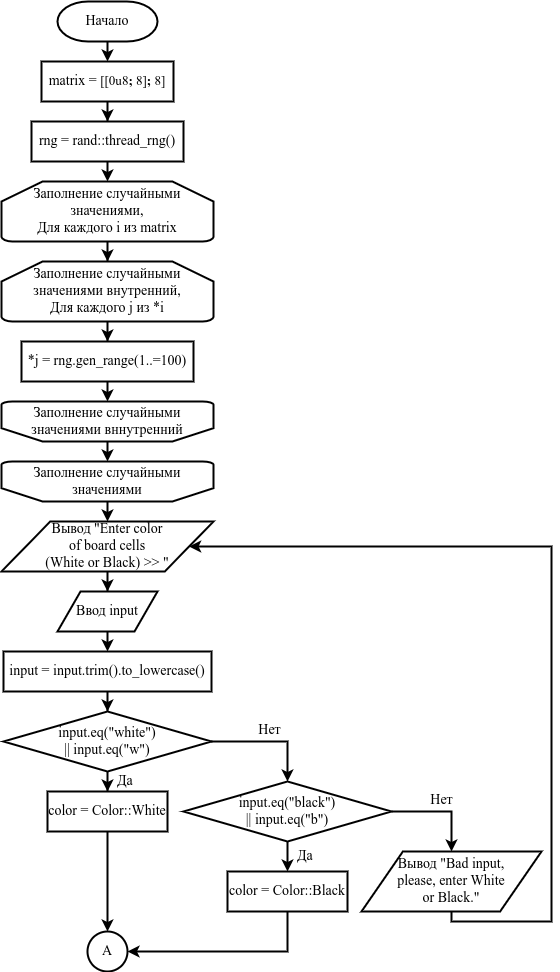
\includegraphics[width=0.85\textwidth]{scheme-main-part1}
\end{figure}

\begin{figure}[H]
	\caption{Блок-схема программы, часть 2}
	\label{fig:scheme-main-part2}
	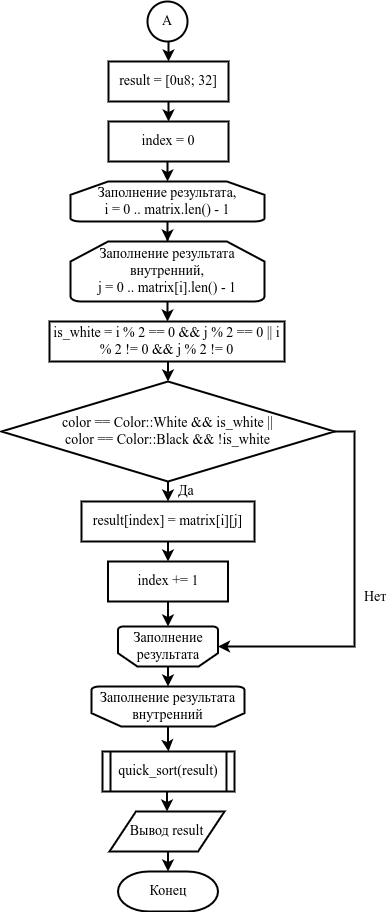
\includegraphics[width=0.55\textwidth]{scheme-main-part2}
\end{figure}

\begin{figure}[H]
	\caption{Блок-схема процедуры quick\_sort}
	\label{fig:scheme-quicksort}
	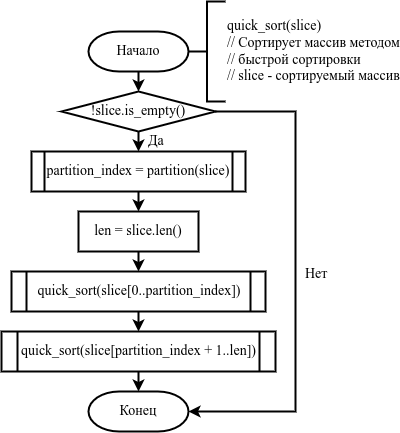
\includegraphics[width=0.7\textwidth]{scheme-quicksort}
\end{figure}
\begin{figure}[H]
	\caption{Блок-схема функции partition}
	\label{fig:scheme-partition}
	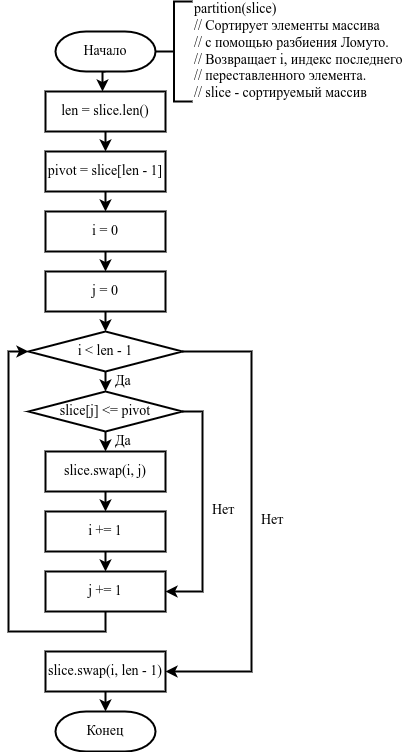
\includegraphics[width=0.7\textwidth]{scheme-partition}
\end{figure}

\section{Код программы}
Код программы на языке программирования Rust представлен \cref{lst:code}.

\setstretch{1}
\lstinputlisting[caption={Код программы},label=lst:code]{matrix/src/main.rs}
\setstretch{1.5}

\section{Примеры тестирования}
Было проведено тестирование программы, которое показало, что программа работает корректно. Результаты тестирования представлены \cref{lst:test1,lst:test2,lst:test3}.
\setstretch{1}
\lstinputlisting[caption={Тестирование черных клеток},label=lst:test1]{test1.txt}
\lstinputlisting[caption={Тестирование белых клеток},label=lst:test2]{test2.txt}
\lstinputlisting[caption={Тестирование обработки некорректного ввода},label=lst:test3]{test3.txt}
\setstretch{1.5}

\chapter{Выводы}
В ходе работы была разработана блок-схема алгоритма и написана программа обработки данных. При этом были проконтролированы типы и диапазоны вводимых данных, а также была предусмотрена обработка других исключительных ситуаций. Блок-схема была изображена по ГОСТу.

\chapter{Информационный источник}
\textbf{Смирнов, С. С.} Информатика : Методические указания по выполнению практических работ / С. С. Смирнов, Д. А. Карпов. -- Москва : МИРЭА -- Российский технологический университет, 2020. -- 102 с.

\end{document}
